Como ya se trato anteriormente \ROOT \footnote{Página del Proyecto: \href{https://root.cern.ch}{https://root.cern.ch}}~ es un ``framework'' para el procesamiento de datos, nacido en el \CERN, dedicado principalmente para la investigación sobre física de altas energías. Todos los días, miles de físicos utilizan aplicaciones \ROOT ~para analizar sus datos o realizar simulaciones, entre sus utilidades encontramos:
\begin{itemize}
\item \textbf{Guardar datos:} compactación en forma binaria comprimida en un archivo de extensión $\mathbf{*.root}$, siendo archivos autodescriptivos, por lo que facilita obtener información sobre los modelos utilizados para describirlos. Su característica principal es ser un contenedor de datos llamado árbol, con sus subestructuras ramas (``branch'') y hojas (``leave''). Un árbol puede verse como una ventana deslizante a los datos sin procesar, tal como se almacenan en un archivo. Los datos de la siguiente entrada en el archivo se pueden recuperar avanzando el índice en el árbol. Esto evita los problemas de asignación de memoria asociados con la creación de objetos y permite que el árbol actúe como un contenedor liviano mientras se maneja el almacenamiento.

\item \textbf{Acceso a los datos:} se accede a los datos guardados en uno o varios archivos \ROOT ~ desde la web o sistemas de entrega de archivos a gran escala. Los árboles \ROOT ~ distribuidos en varios archivos se pueden encadenar y acceder como un objeto único, lo que permite bucles sobre grandes cantidades de datos.

\item \textbf{Mina de datos:} posee potentes herramientas matemáticas y estadísticas para operar con sus datos, todo sobre $\mathbf{C++}$, pŕeparado para el procesamiento en paralelo cuando se requiera la manipulación de los mismos. Permite la generación de cualquier distribución estadística y modelados, logrando simular sistemas complejos.

\item \textbf{Gráfica resultados:} los datos se pueden mostrar con histogramas, diagramas de dispersión, funciones de ajuste ya integradas como herramientas en su biblioteca.

\item \textbf{Ejecución interactiva o creación de aplicaciones:} Puede usar el intérprete Cling $\mathbf{C++}$ para sus sesiones interactivas y para escribir macros, o puede compilar su programa para que se ejecute a toda velocidad, siempre dando la posibilidad de crear una interfaz gráfica de usuario.
\end{itemize}

Hay muchas herramientas creadas a partir de \ROOT, entre ellas se pueden destacar el generador de Monte-Carlo Madgraph, y entre las herramientas interactivas a \textbf{EVE}.


%\begin{figure}[ht!]
%    \centering
%    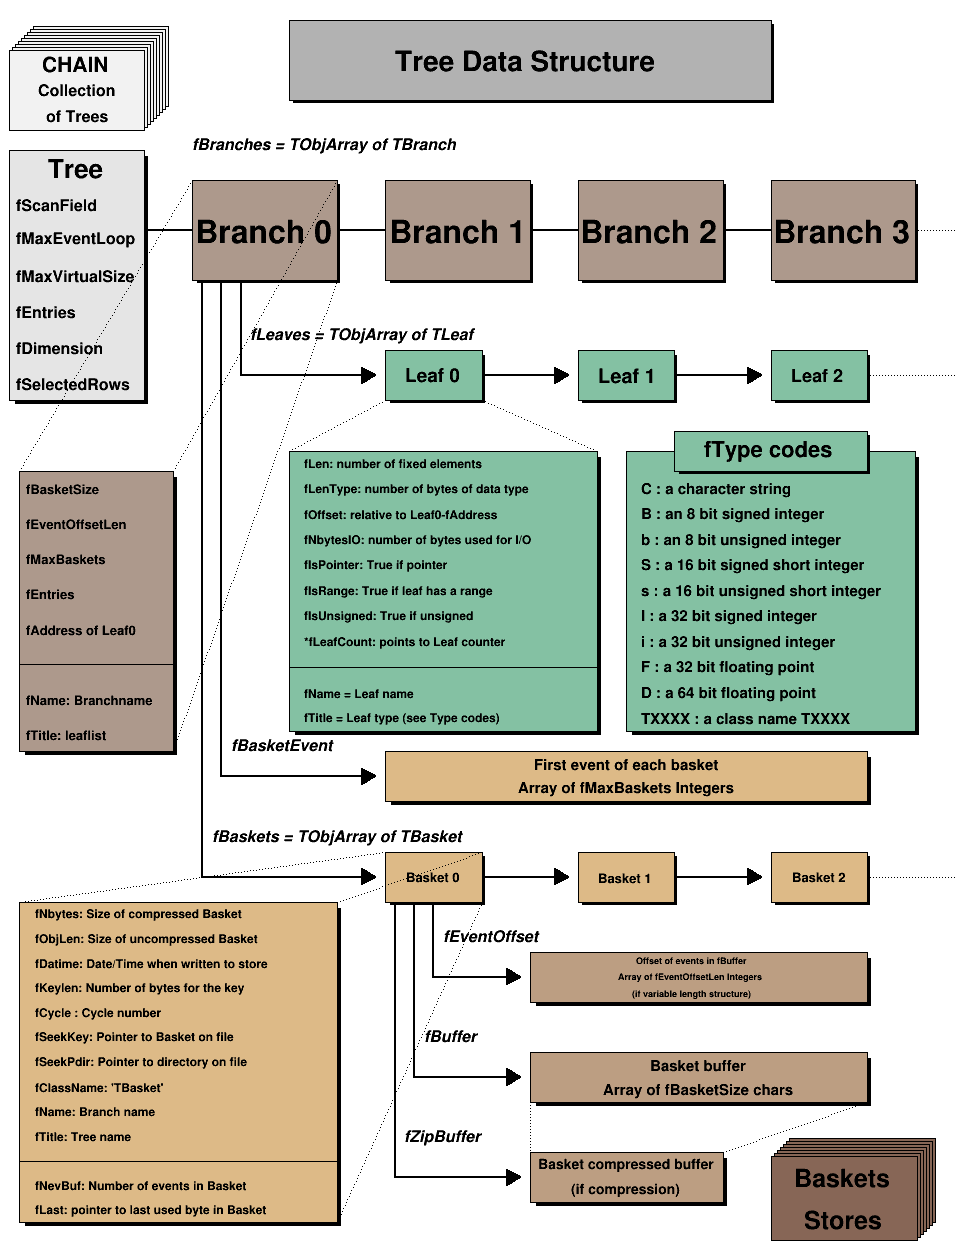
\includegraphics[width=0.84\textwidth]{Analisis_y_Resultados/imagenes/trees_root.png}
%    \caption{Estructura de los datos en forma de árbol.}
%    \label{fig:trees_root}
%\end{figure}